\chapter{Introduzione}
\section{La moltiplicazioni tra matrici}
Per moltiplicazioni tra matrici si intende il prodotto tra righe e colonne tra due matrici. Questo prodotto, possibile sotto certe condizioni, da luogo ad un'altra matrice.

Esistono vari tipi di matrici: vettori, quadrate, rettangolari. Ovviamente si possono moltiplicare questi diversi tipi tra di loro a patto che sussistano delle condizioni sulle loro dimensioni.

Si pu\`{o} eseguire il prodotto tra A e B a patto che il numero delle colonne della matrice A (prima matrice) sia uguale al numero delle righe  di B (seconda matrice).

Il prodotto AB avr\`{a} il numero di righe di A (prima matrice) ed il numero di colonne di B (seconda matrice).

Dunque il prodotto tra due matrici quadrate delle stesse dimensioni \`{e} sempre possibile.

Esempi:

A[4 x 5] x B[4 x 2] = C[4 x 2]

A[4 x 4] x B[4 x 6] = C[4 x 6]

A[4 x 4] x B[4 x 4] = C[4 x 4]

Il funzionamento del prodotto tra matrici \`{e} spiegato dalla figura \ref{fig:diagram}.

\begin{figure}[htbp]
    \begin{center}
        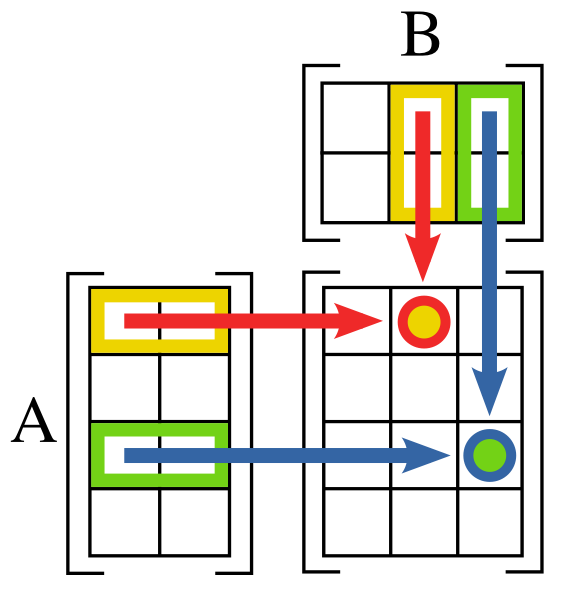
\includegraphics[width=5cm]{immagini/matrix_multiplication_diagram.png}
    \end{center}
    \caption{Diagramma della moltiplicazione}
    \label{fig:diagram}
\end{figure}

Il diagramma mostra il caso in cui A \`{e} 4 x 2 e B \`{e} 2 x 3, e si voglia calcolare l'elemento $(C)_{12} = (AB)_{12}$ (figura \ref{fig:formula_c}) della matrice prodotto C = A x B, di dimensioni 4 x 3.

\begin{figure}[htbp]
    \begin{center}
        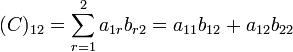
\includegraphics[width=10cm]{immagini/matrix_multiplication_formula_c.png}
    \end{center}
    \caption{Formula per calcolare $(C)_{12}$}
    \label{fig:formula_c}
\end{figure}

Pi\`{u} generalmente possiamo esprimere la moltiplicazioni di due matrici con la figura \ref{fig:matrix_multiplication_generic} dove ogni elemento della matrice C \`{e} calcolato utilizzando la formula in figura \ref{fig:matrix_multiplication_generic_formula}.

\begin{figure}[htbp]
    \begin{center}
        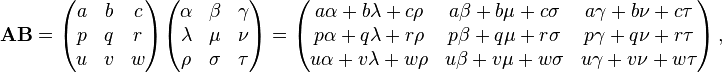
\includegraphics[width=15cm]{immagini/matrix_multiplication_generic.png}
    \end{center}
    \caption{Esempio di prodotto tra matrici}
    \label{fig:matrix_multiplication_generic}
\end{figure}

\begin{figure}[htbp]
    \begin{center}
        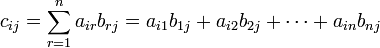
\includegraphics[width=10cm]{immagini/matrix_multiplication_generic_formula.png}
    \end{center}
    \caption{Formula generica per calcolare $c_{ij}$}
    \label{fig:matrix_multiplication_generic_formula}
\end{figure}

\section{Parallelizazione}
La moltiplicazioni tra matrici appartiene a quella classe di problemi che possono essere parallelizzati o ottimizzati.
Esistono molte ottimizzazioni come ad esempio: Strassen, Coppersmith-Winograd, etc\ldots (vedi figura \ref{fig:matrix_algo})

\begin{figure}[htbp]
    \begin{center}
        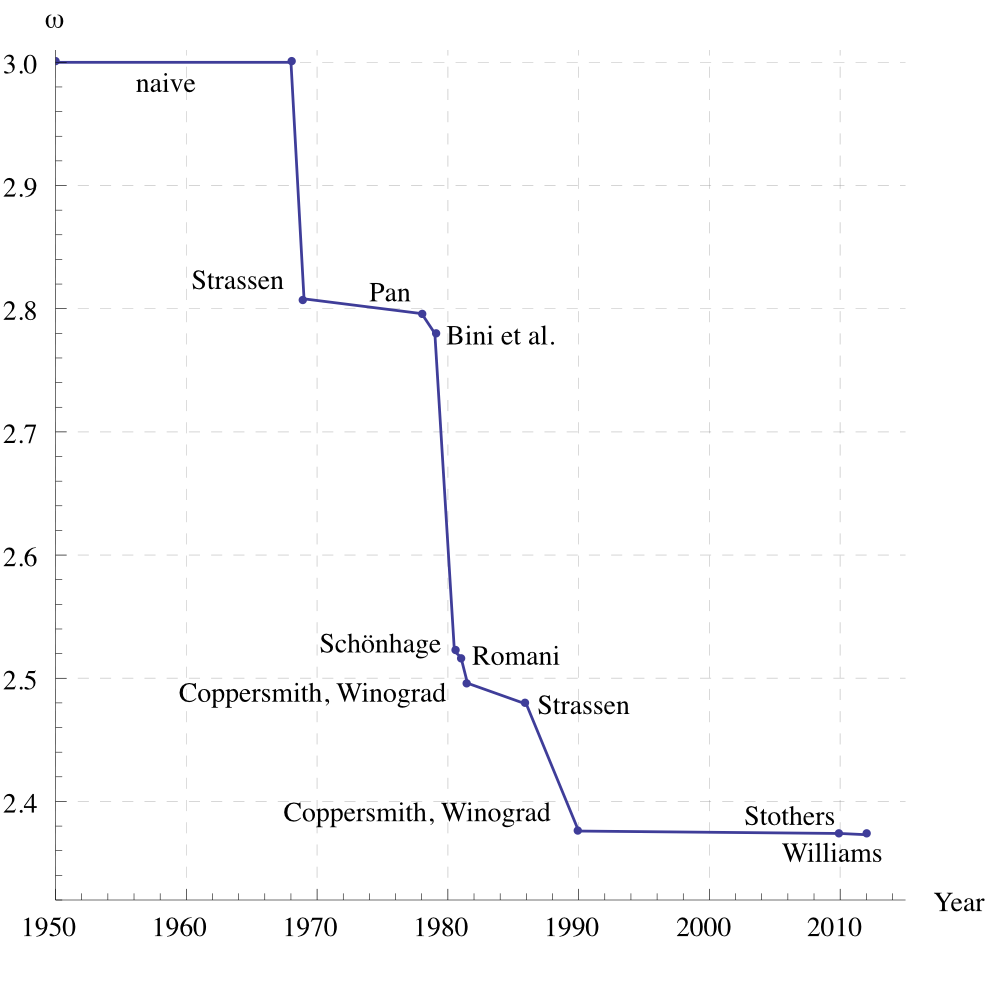
\includegraphics[width=7cm]{immagini/matrix_algorithms.png}
    \end{center}
    \caption{Ottimizzazioni di algoritmi di moltiplicazioni tra matrici nel tempo}
    \label{fig:matrix_algo}
\end{figure}

Per quanto riguarda la parallelizzazione ci sono algoritmi che sfruttano memoria condivisa mentre altri che sono distribuiti decomponendo il problema in sottoproblemi da eseguire localmente. Questo tipo di approccio porta con se diverse problematiche come overhead di comunicazione, decomposizione del problema e scambio di informazioni tra i vari nodi.
Senza scendere troppo nei dettagli dei vari algoritmi distribuiti, possiamo trovare l'algoritmo di Cannon spiegato nel prossimo capitolo ed utilizzato per lo sviluppo dell'applicazione.
